\chapter{Aachen-Turbine}
\label{cha:aachen}
Zur Analyse der verschiedenen Wirkungsgraddefinitionen wurde die Aachen-Turbine, eine Turbine mit Schaufeln ohne Krümmung in Radialrichtung, simuliert. In diesem Kapitel wird zunächst die Geometrie und die durchgeführte Gitterstudie vorgestellt. Danach werden die ermittelten Wirkungsgrade miteinander verglichen und Unterschiede vorgestellt.
\section{Geometrie}
\label{sec:aachengeo}
  \begin{figure}[htbp]
	\centering
	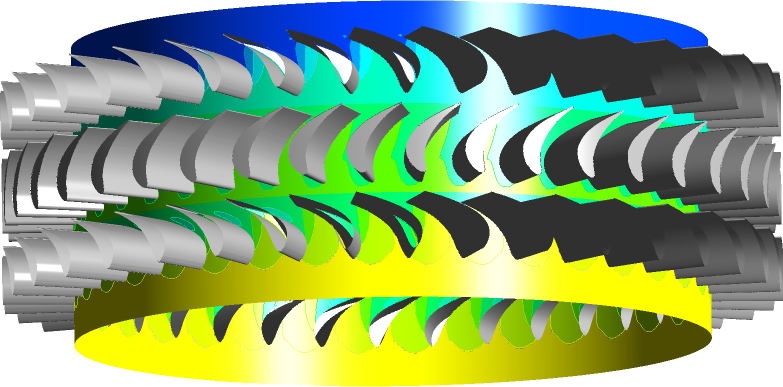
\includegraphics[width=0.8\textwidth]{AachenTurbine_trans.png}
	\caption{Aachen-Turbine} \label{fig:imgAachenTurbine}
\end{figure} 
Die verwendete Geometrie basiert auf der Aachen-Turbine, die auch in den Untersuchungen von J. Yao, R. L. Davis, J. J. Alonso und A. Jameson\cite{ufi2001YaoDavis} 
verwendet wurde. Es werden dabei nur 1,5 Stufen berechnet, um den Rechenaufwand der Simulationen gering zu halten und den Vergleich der Wirkungsdefinitionen auch für diesen Aufbau möglich zu machen. Die Geometrie der Aachen-Turbine mit Gitter ist in Abbildung \ref{fig:aachengebiet} zu sehen. 
\begin{figure}[htbp]
	\centering
	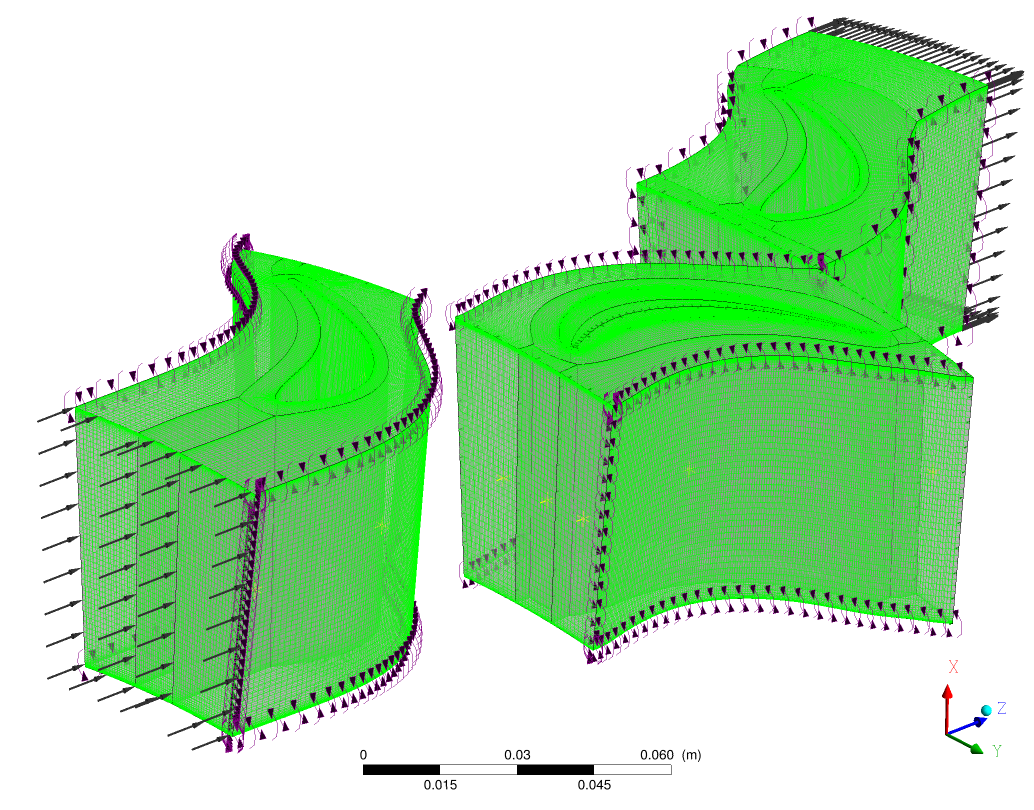
\includegraphics[width=0.7\textwidth]{aachenmitgitter.png}
	\caption{Eine dreidimensionale Ansicht der Aachen-Turbine mit Gitter}
	\label{fig:aachengebiet}
\end{figure}
Die Aachen-Turbine besteht aus zwei Statoren und einem Rotor. Die erste Domäne als Stator mit Einstrom, die mittlere Domäne als Rotor und die letzte Domäne als zweiter Stator mit Ausstrom. Die Grenzen oben und unten stellen Shroud und Hub dar. Links und rechts herrschen periodische Randbedingungen. Die Statoren sind jeweils durch ein Interface mit dem Rotor verbunden. Die Anzahl an Schaufeln in Stator und Rotor sind aus Tabelle \ref{tab:aachenabmessungen} zu entnehmen.\newline
\begin{table}[htbp]
\centering
\label{tab:aachenabmessungen}
\caption{Schaufelzahlen in Stator und Rotor}
\begin{tabular}{ c| c}
\# Schaufeln in Stator&\# Schaufeln in Rotor\\
\hline
36&41\\
\end{tabular}
\end{table}
Im folgenden Abschnitt wird der gewählte Betriebspunkt näher beschrieben.
%________________________________________________________
\section{Betriebspunkt}
\label{subsec:aachensetup}
Um den Betriebspunkt für die Simulationen dieser Arbeit festzulegen, werden zur Vergleichbarkeit die Randbedingungen der Arbeit \glqq Unsteady Flow Investigations in an
Axial Turbine Using the Massively
Parallel Flow Solver TFLO\grqq \, \cite{ufi2001YaoDavis} zur Analyse der Aachen-Turbine übernommen. Diese sind der folgenden Tabelle \ref{tab:aachensetup} zu entnehmen.
\begin{table}[H]
\centering
\caption{Betriebspunkt} \label{tab:aachensetup}
\begin{tabular}{ c| c| c| c}
$T_{t_{Inlet}}$&$p_{t_{Inlet}}$&$Massenstrom$&$n_{Rotor}$\\
\hline
$305 \, K$&$\approx152.000 \, Pa$&$7 \, \frac{kg}{s}$&$3500 \, \frac{rev}{min}$\\
\end{tabular}
\end{table}
Der Totaldruck am Inlet wird als Druckprofil, siehe Abbildung \ref{fig:ptinlet}, entsprechend den Daten von \cite[p. 4]{ufi2001YaoDavis} angenommen.
In den verschiedenen Aufgabenteilen dieser Arbeit werden die Eintrittsbedingungen jedoch auch verändert, um zum Beispiel den Einfluss inhomogener Eintrittsbedingungen oder höherer Temperaturen zu untersuchen.

\begin{figure}[htbp]
	\centering
	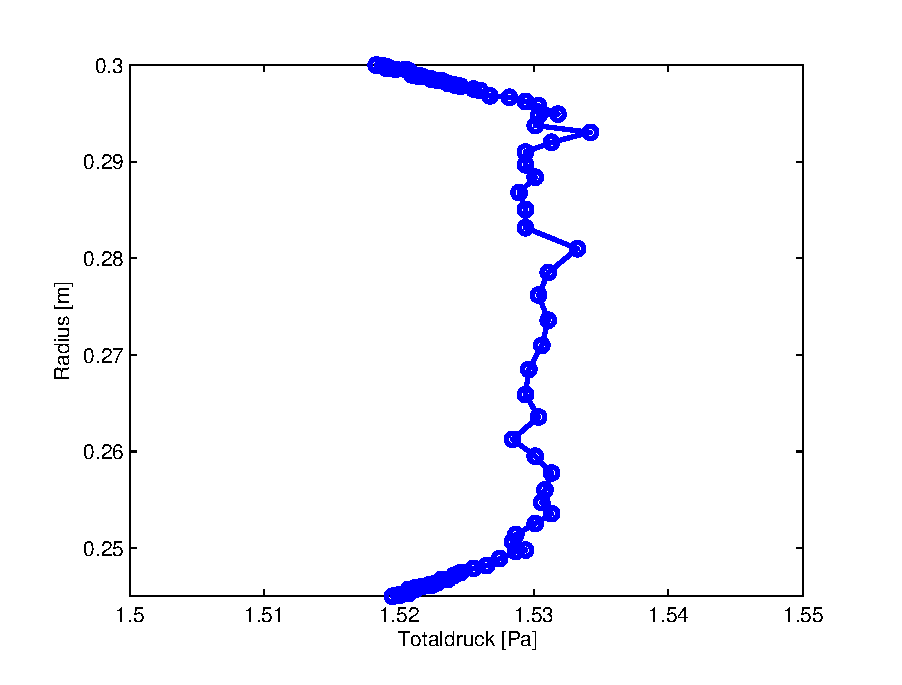
\includegraphics[width=0.8\textwidth]{PtInlet.eps}
	\caption{Totaldruck Profil Inlet} \label{fig:ptinlet}
\end{figure}


\section{Strukturiert}
Im Folgenden wird beschrieben, wie das strukturierte Netz der Aachen-Turbine erstellt wurde. Da das Netz Einfluss auf die numerische Konvergenz der Lösungsverfahren, auf die Qualität der Lösung, auf die Auflösung und damit auch auf den Diskretisierungsfehler hat, ist ein gutes Netz von großer Bedeutung. Deshalb wurde eine Netzstudie - basierend auf einem Referenzgitter – durchgeführt und anschließend das bestmögliche Netz in Bezug auf Qualität vs. geringe Anzahl an Gitterzellen ausgewählt. 

\subsection{Erstellung des Gitters}

Zunächst wurde das Referenzgitter erstellt. Dazu wurde die Geometrie der Aachen-Turbine mittels des strukturierten Multi-Block Netzgenerators AutoGrid5 vernetzt. Dieser ist speziell für die Vernetzung von Turbomaschinen ausgelegt. 
Da die uns zur Verfügung stehende Vorlage der Aachen-Turbine die 1,5 Stufen zusammenhängend beinhaltete, erzeugten wir zu Beginn jeweils einzelne Gitter für Stator1, Rotor und Stator2 um diese später in CFX verwenden zu können. Hierbei wurde jeweils erst ein Vernetzungsdurchlauf basierend auf den voreingestellten Standartwerten durchgeführt und anschließend manuell optimiert. Für eine ausreichend gute Netzqualität dürfen bestimmte Netzkriterien nicht verletzt werden. Andernfalls kann es sein, dass die Lösung nicht, oder nur schlecht konvergiert. In unserem Fall haben wir darauf geachtet, dass wir keine negativen Kontrollvolumina haben, dass die kleinsten Winkel in einer Zelle größer 20° sind, dass das Expansionratio - welches das Volumenverhältnis zweier Zellen beschreibt – kleiner als 2.3 ist und dass das Aspectratio – welches das Verhältnis von längster zu kürzester Seite einer Zelle angibt – unter 1500 ist. Variiert wurden hauptsächlich die Anzahl und die Verteilung der Zellen in der B2B Ansicht. Diese stellt einen Querschnitt durch die Schaufel dar. In radialer Richtung wurde die Zellenverteilung im „flowpath“ angepasst. 

\subsection{Spaltverfeinerung}

Zur Bestimmung der Gitterauflösung im Spalt des Rotors wurde zudem die Anzahl der Zellen im Spalt variiert. Es stellte sich heraus, dass im Vergleich zum ursprünglichen Gitter mehr Zellen hinzugefügt werden mussten, da die Auflösung nicht fein genug war und man Änderungen im Vergleich zur gröberen Auflösung sah.  In den Abbildungen \ref{effSpalt1} und \ref{effSpalt15} ist die Gitterstudie für den Spalt mit 1 und 1,5 Stufen dargestellt. \todo welches Gitter ausgewählt, 3.?


\begin{figure}[htbp]
	\centering
	\label{effSpalt1}
	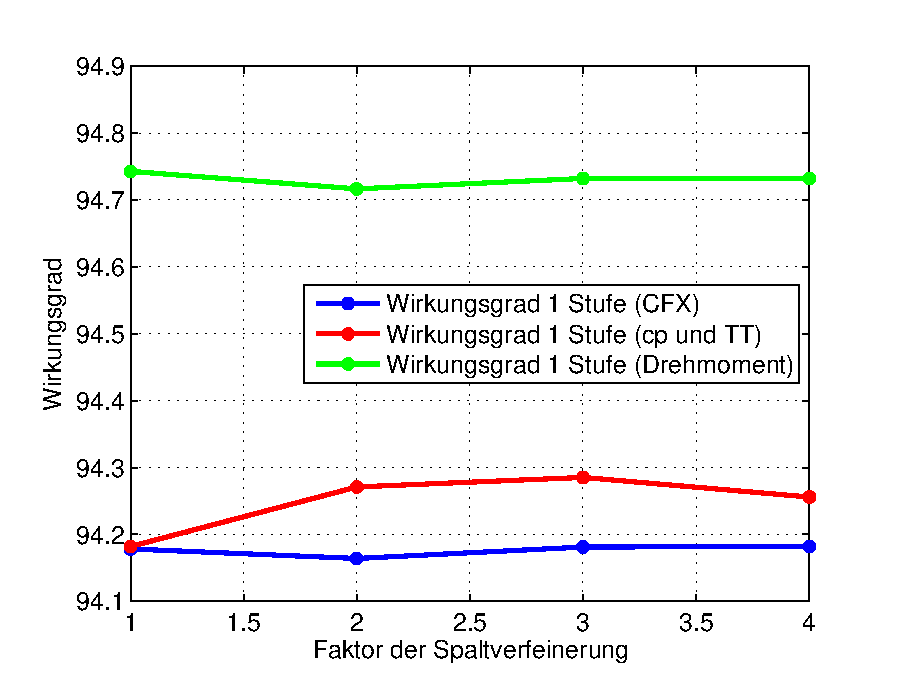
\includegraphics[width=0.7\textwidth]{efficiencySpalt1Stufe.eps}
	\caption{Gitterstudie des Spalts für eine Stufe}
\end{figure}

\begin{figure}[htbp]
	\centering
	\label{effSpalt15}
	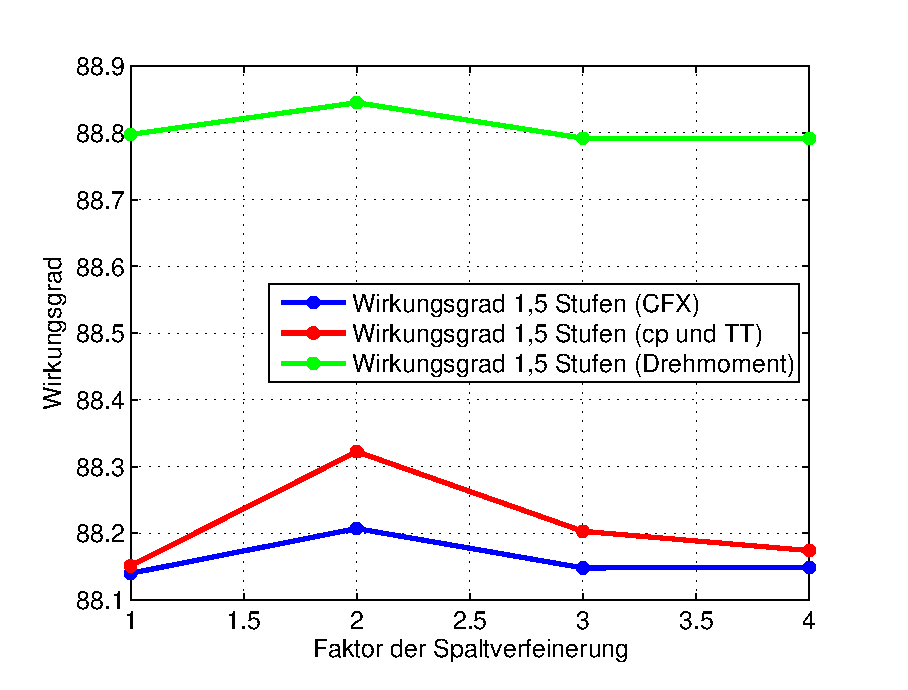
\includegraphics[width=0.7\textwidth]{efficiencySpalt15Stufen.eps}
	\caption{Gitterstudie des Spalts für 1,5 Stufen}
\end{figure}

\subsection{Einstellen der Grenzschichtdicke}
Außerdem musste noch die Grenzschichtdicke, bzw. das y-plus eingestellt werden. Die Strömung wurde bis in die viskose Unterschicht aufgelöst, sodass die Auflösung in Wandnähe im Bereich der kleinsten Wirbel liegt. Das Verhältnis der Grenzschichtdicke zu den kleinsten Wirbeln sollte kleiner als 1 sein. \todo Formel einfügen. Um das korrekte y-plus zu bestimmen, haben wir die Werte in AutoGrid für den Wandabstand sowohl auf dem Schaufelrand im B2B-Layer, als auch an Hub und Shroud variiert.  Anschließend haben wir eine Simulation in CFX durchgeführt und dann die Verteilung des y-plus-Wertes über die Schaufel hinweg visualisiert und ausgewertet. Schließlich kamen wir zu dem Ergebnis, dass die optimale Grenzschichtdicke für den Rotor bei $2e-6$ im Flowpath an Hub und Shroud und bei $1.5e-6$ am Blade liegt. Die kompletten Werte sind in Tabelle \ref{cellWidths} zu sehen. Über die komplette Schaufel betrachtet liegen die y-plus-Werte in einem Bereich von $0.3 \leq y^+ \leq 3$ nahezu überall. Da man nur wenige Stellschrauben zur Beeinflussung dieses Wertes in AutoGrid hat, ist dieser Wertebereich zufriedenstellend, zumal die Mehrheit der Werte im Bereich von $0.7 \leq y^+ \leq 1.2$  liegt, wie in Abb. \ref{imgYplusWerte} zu sehen ist. 

\begin{table}[t]
\centering
\begin{tabular}[t]{cccc}
\toprule
 Cell width  & Stator1 & Rotor & Stator2  \\
\midrule
Cell width at Hub & 2.7e-6 & 2e-6 & 1.4e-6\\
Cell width at Shroud & 2.7e-6 & 2e-6 & 1.4e-6 \\
Cell width at Wall (Blade) & 1.56e-6 & 1.5e-6 & 1.7e-6 \\
\bottomrule
\end{tabular}
\caption{Zellgrößen an der Wand für Rotor und die Statoren}
\label{cellWidths}
\end{table}

\begin{figure}[htbp]
	\centering
	\label{imgYplusWerte}
	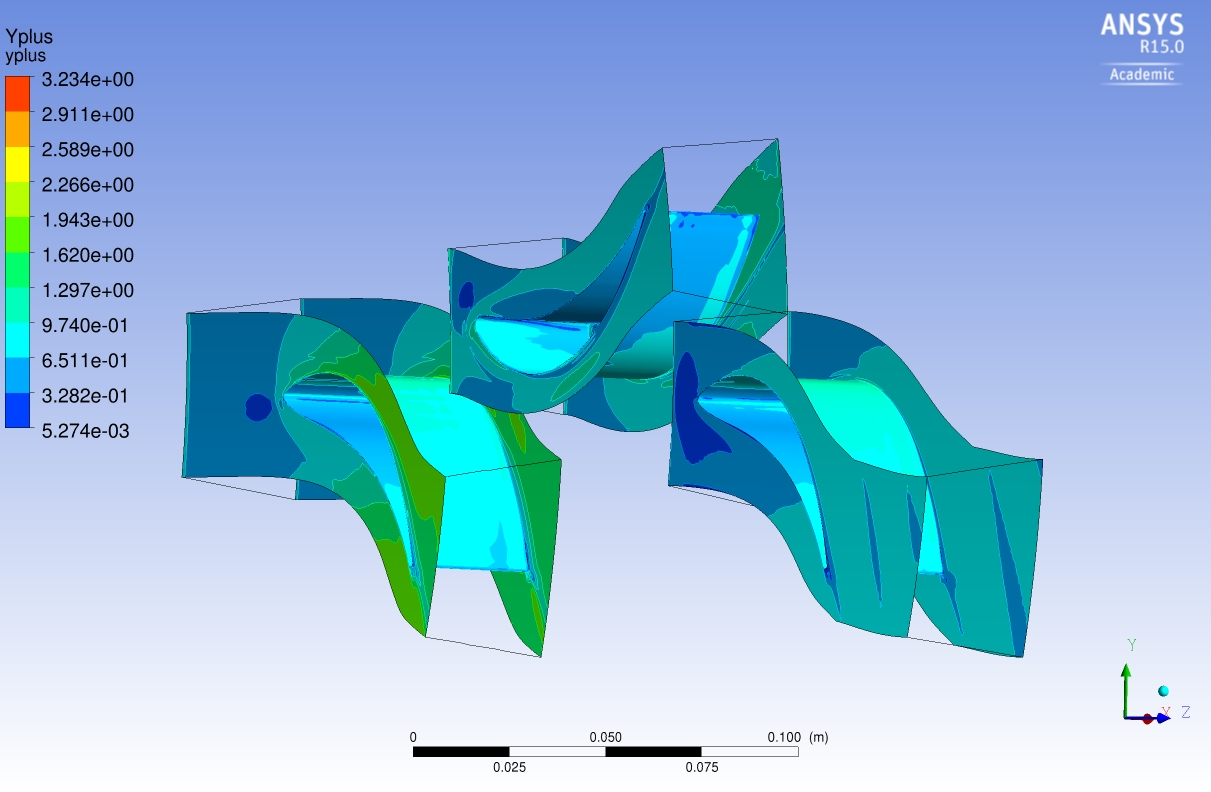
\includegraphics[width=0.7\textwidth]{yPlus.jpg}
	\caption{$y^+$-Verteilung über die komplette Stufe}
\end{figure}

\subsection{Durchführung der Netzstudie}

Nachdem nun ein Referenzgitter mit guter Gitterqualität und korrekter Grenzschichtdicke vorhanden war, konnte die eigentliche Netzstudie durchgeführt werden um die minimale Auflösung zu bestimmen, die das Netz haben muss, damit die Lösung netzunabhängig ist. Hierzu wurde das Referenzgitter sowohl gröber aufgelöst, als auch verfeinert und dann der Einfluss auf verschiedene Größen, die z.B. die Wirkungsgrade verglichen. Sobald sich dieser im Vergleich zum nächst feineren, bzw. nächst gröberen Gitter kaum noch ändert, ist die Lösung von der Gitterdiskretisierung unabhängig. 
Insgesamt wurden 7 verschiedene Verfeinerungsstufen erstellt und simuliert. Das Referenzgitter hat jeweils knapp 1 Million Zellen für Rotor und die Statoren. Zunächst wurde versucht, die Zellenanzahl zu verdoppeln. Dazu wurde die Auflösung in allen drei Raumrichtungen mit $\sqrt[3]{2}$ multipliziert um insgesamt einen Faktor von 2 zu erlagen. Dies wurde dann nochmal wiederholt, um einen Faktor 4 gegenüber dem Referenznetz zu erreichen. Außerdem wurde das Referenznetz auf die halbe Zellenanzahl halbiert. Mit den Ergebnissen, dieser 4 Simulationen wurde bereits versucht, eine Aussage über die Netzunabhängigkeit zu treffen. Allerdings war hier noch nicht ganz ersichtlich, welches Netz hier genommen werden konnte, da die Unterschiede noch zu groß waren. Allerdings sah das 2x Gitter schon sehr gut aus. Daraufhin führten wir noch drei weitere Simulationen durch, jeweils mit den Auflösungen 1.3x, 1.5x und 3x in Bezug zum Referenzgitter. Nun war zu erkennen, dass das Netz mit der doppelten Auflösung praktisch unabhängig war, sodass wir dieses als unser Gitter für die nachfolgenden Rechnungen definieren konnten. 
\todo Kenngrößen des Gitters hinschreiben + Plots einfügen


\subsection{Fillets}

In realen Turbinen befinden sich an der Schaufel am Übergang zum Randbereich sogenannte Fillets, also Verrundungen, um bessere Strömungseigenschaften zu erhalten, Ablöseblasen zu vermeiden und bessere Festigkeitseigenschaften zu erhalten. Daher wurde auch eine Simulation der Aachen-Turbine mit Fillets durchgeführt, das Netz ist in Abb. \ref{imgFillet1} zu sehen. Jedoch ergab sich das Problem, dass nur sehr kleine Fillets erstellt werden konnten, da die Statoren eine „Delle“ an der Vorderkante aufweisen, wie in Abb. \ref{imgFilletDelle} zu sehen ist und daher ab einem bestimmten Radius negative Kontrollvolumen durch die Fillets entstehen. Jedoch wurde eine Simulation mit einem Fillet des Radius 0.00055 durchgeführt. Es hat sich herausgestellt, dass die Gitterqualität wesentlich schlechter wurde, da mehr schrägwinklige Zellen im Filletbereich notwendig wurden. Allerdings wurde auch der y-plus-Wertebereich etwas besser, da sehr kleine und sehr große Werte verschwanden.     

  \begin{figure}[htbp]
	\centering
	\label{imgFillet1}
	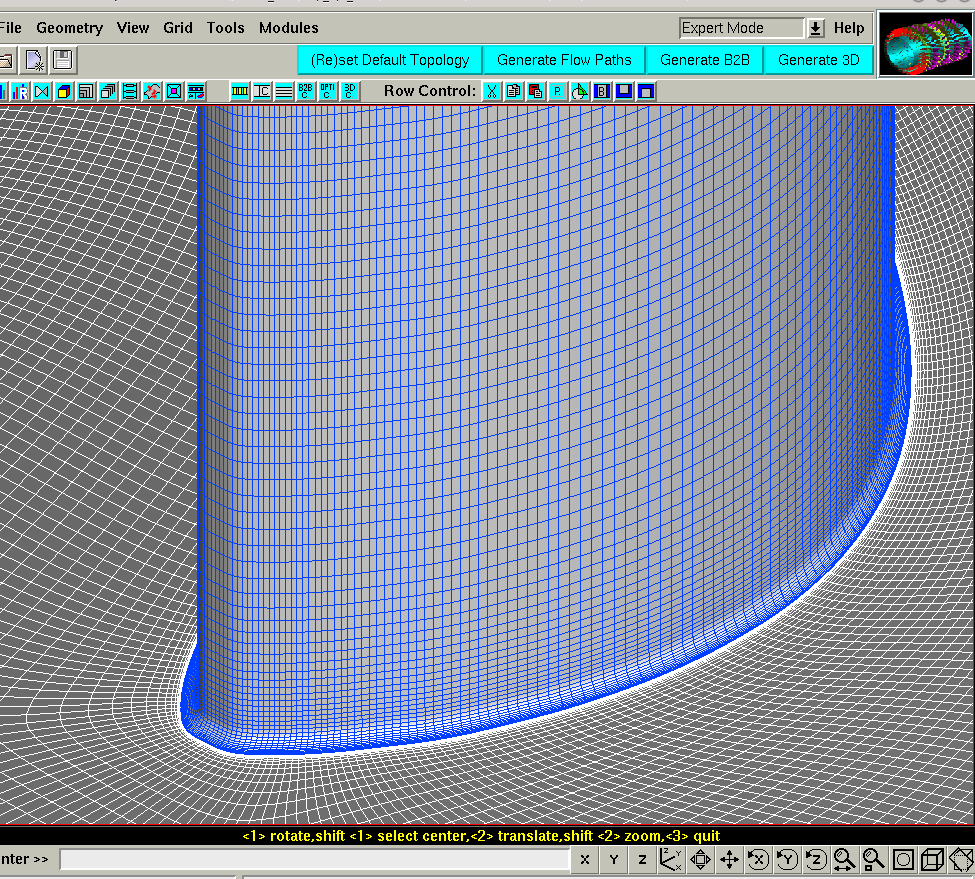
\includegraphics[width=0.7\textwidth]{fillet0_00055.png}
	\caption{Netz mit Fillet der Größe 0.00055}
\end{figure} 

  \begin{figure}[htbp]
	\centering
	\label{imgFilletDelle}
	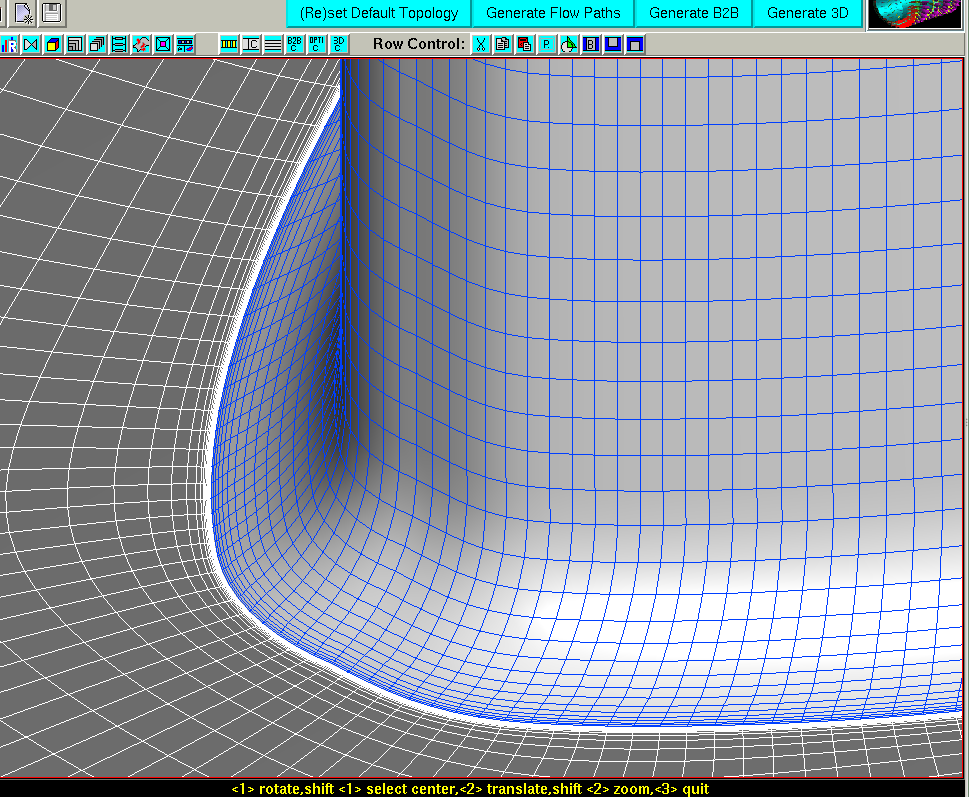
\includegraphics[width=0.7\textwidth]{filletDelle.png}
	\caption{Delle in der Statorgeometrie}
\end{figure} 
\section{Unstrukturiertes Gitter}
Um generelle Unterschiede zwischen einem strukturierten und unstrukturierten Gitter festzustellen, wurden zusätzlich Berechnungen mit einem unstrukturierten Gitter durchgeführt.

\subsection{Aufgetretene Probleme}
Für den zweiten Stator liegt kein CAD-File, lediglich eine Netzdatei vor. Somit war es nicht möglich ein unstrukturiertes Gitter für diesen zu erstellen. Für die Berechnungen wurde daher das Gitter der Aachen-Turbine teilweise unstrukturiert und strukturiert betrachtet.\\
Die Erstellung der unstrukturierten Gitter war aufgrund von Lizenzproblemen nicht immer möglich, was die Anzahl der durchgeführten Simulationen eingrenzt.
\subsection{Erstellung des Gitters}
Das unstrukturierte Gitter wurde mit Centaur erstellt. Zunächst wurde ein Referenzgitter mit den Standardwerten gebildet. Für das Einstellen von $y^+$ wurde zunächst der gleiche Wandabstand wie im Falle des strukturierten Gitters verwendet. Nach einem ersten Test wurde dieser im Rotor verringert. Die Verteilung von $y^+$ des ersten Stators und Rotors ist in Abbildung \ref{yplusunstrukturiert} dargestellt.
\begin{figure}[htbp]
	\centering
	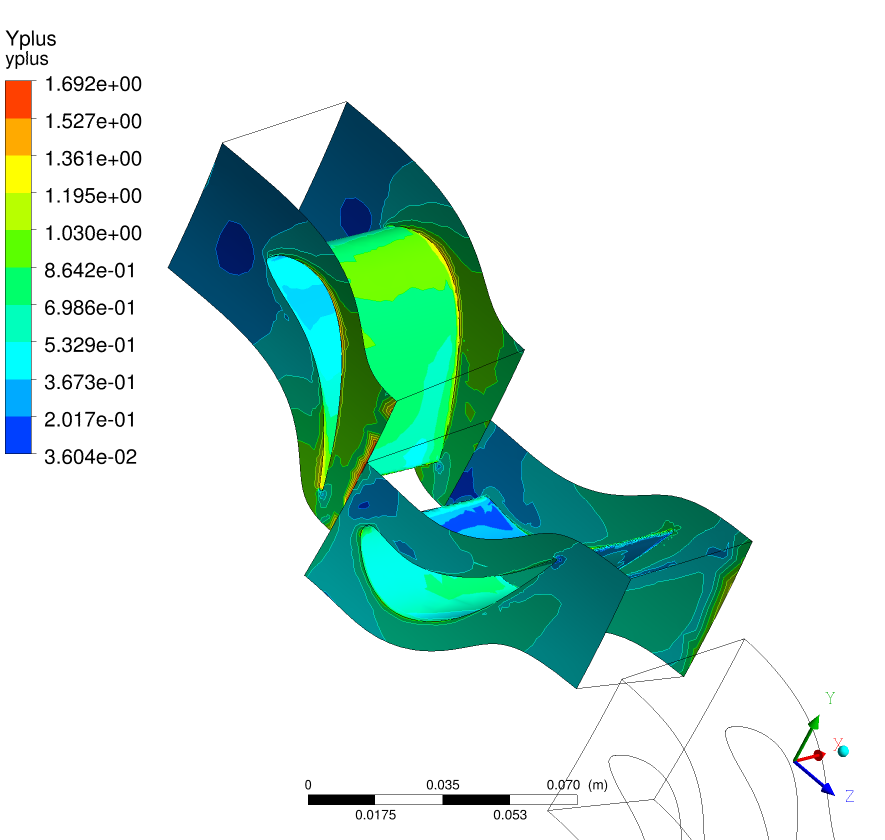
\includegraphics[width=0.7\textwidth]{yplusunstrukturiert.png}
	\caption{$y^+$ des unstrukturierten Gitters} \label{yplusunstrukturiert}
\end{figure}
\subsubsection{Verwendung von Sources}
Um das Gitter lokal an bestimmten Stellen zu verfeinern wurden  sogenannte Sources mit Hilfe Centaur eingeführt.
Eine davon regelt die unterschiedlichen Wandabstände von Schaufel, Nabe und Gehäuse.\\
Eine weitere Source verfeinert die Zellen im Nachlauf der Schaufel relativ zu den umliegenden Zellen um den Faktor $c = 0.8$.

\subsection{Gitterstudie}
Zuerst wurde der Spalt des Rotors wie beim strukturierten Gitter verfeinert. Anschließend wurde eine Gitterstudie mit verschiedenen Verfeinerungsstufen, siehe Tabelle \ref{tab:verfeinerungenunstrukturiert}, durchgeführt. In den Abbildungen \ref{fig:gitterunstrukturiert1stufe} und \ref{fig:gitterunstrukturiert15stufen} ist der Wirkungsgrad in \% über die Verfeinerungsstufen aufgetragen. Es ist zu erkennen, dass die Wirkungsgrade weiterhin in Abhängigkeit der Kontrollvolumenzahl steigen. Damit eine netzunabhängige Lösung ermittelt werden kann, müssten weitere Verfeinerungsstufen zwischen 2 und 3 und größer 3 gerechnet werden, bis kein Ansteigen oder Absinken mehr zu erkennen ist. Dies war aufgrund von Lizenzproblemen nicht möglich.\\
Für die Berechnungen mit einem temperaturabhängigen $c_p$ und für die Vergleiche mit dem strukturierten Gitter wurde das feinste Netz verwendet.
\begin{table}[h]
		\centering
		\caption{Verfeinerungsstufen des unstrukturierten Gitters}
	\begin{tabular}{ c| c | c| c| c}
Verfeinerungsstufe	&	Stator 1	&		&	Rotor	&		\\
&	Anzahl Knoten	&	Anzahl Elemente	&	Anzahl Knoten	&	Anzahl Elemente	\\
\hline									
0,5	&	61435	&	174098	&	281782	&	724470	\\
1	&	147399	&	473211	&	638948	&	1741931	\\
2	&	244772	&	880367	&	1007020	&	2835297	\\
\textbf{3}	&	\textbf{1196277}	&	\textbf{6457352}	&	\textbf{1880370}	&	\textbf{6844537}	\\

	\end{tabular}
		\label{tab:verfeinerungenunstrukturiert}
\end{table}
\begin{figure}[htbp]
	\centering
	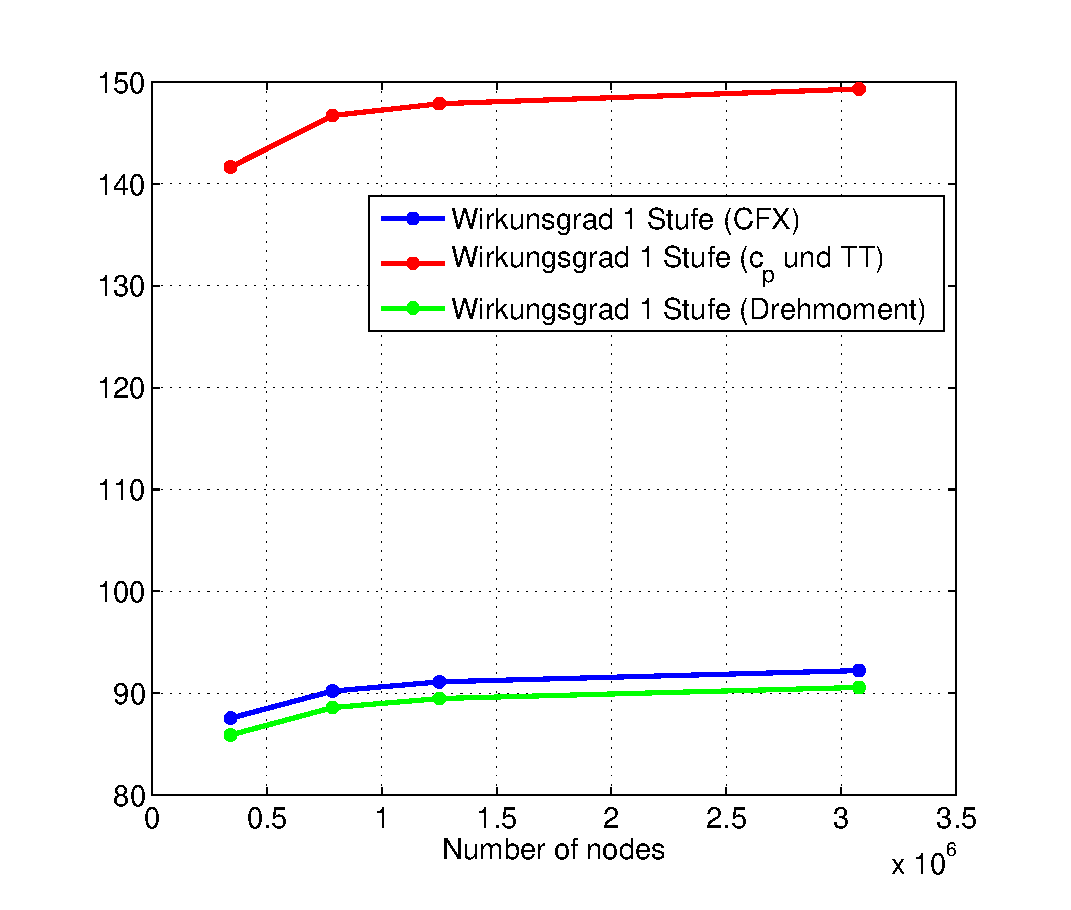
\includegraphics[width=0.7\textwidth]{gitterstudieunstrukturiert1stufe.eps}
	\caption{Gitterstudie des unstrukturierten Gitters für eine Stufe} \label{fig:gitterunstrukturiert1stufe}
\end{figure}

\begin{figure}[htbp]
	\centering
	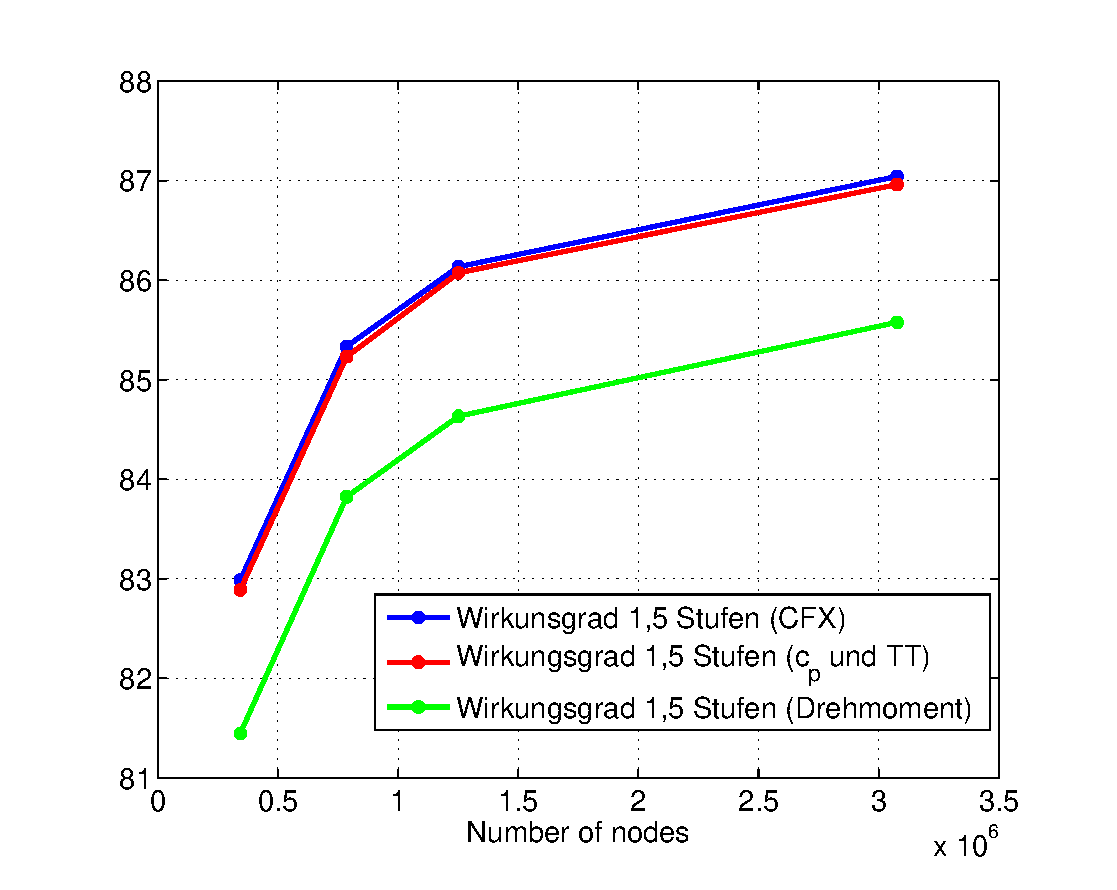
\includegraphics[width=0.7\textwidth]{gitterstudieunstrukturiert15stufen.eps}
	\caption{Gitterstudie des unstrukturierten Gitters für 1,5 Stufen}
	\label{fig:gitterunstrukturiert15stufen}
\end{figure}
\section{Vergleich der Wirkunsgrade}
Bei der Aachen-Turbine ergaben sich je nach Berechnungsart folgende Werte für den Wirkungsgrad:
\begin{table}[H]
	\centering
	\caption{Wirkungsgrad bei der Aachen-Turbine}
	\begin{tabular}{ c| c | c}
Berechnungsformel	&	$\eta_{strukturiert}$	&	$\eta_{unstrukturiert}$	\\
\hline
1 Stufe	&		&		\\
\hline
$\eta_{CFX}$	&	$92,33\%$	&	$92,23\%$	\\
$\eta_{c_p, T_t}$	&	$92,44\%$	&	$92,23\%$	\\
$\eta_{torque}$	&	$92,87\%$	&	$90,58\%$	\\
\hline
1,5 Stufen 	&		&		\\
\hline
$\eta_{CFX}$	&	$86,42\%$	&	$87,05\%$	\\
$\eta_{c_p, T_t}$	&	$86,48\%$	&	$87\%$	\\
$\eta_{torque}$	&	$87.05\%$	&	$85,58\%$	\\

	\end{tabular}
	\label{tab:wgaachen}
\end{table}
In Tabelle \ref{tab:wgaachen} werden die Wirkungsgrade des strukturierten und des unstrukturierten Gitters dargestellt. Diese weichen höchstens um $1,7\%$ voneinander ab. Es ist zu erkennen, dass die Wirkungsgrade im strukturierten Fall bei einer Stufe bis zu zwei Prozentpunkten größer sind. Bei der Betrachtung von 1,5 Stufen ist dagegen zu erkennen, dass die Wirkungsgrade im strukturierten Fall um $0,6$ Prozentpunkte kleiner sind.\\
Dies kann an dem Übergang vom Rotor in den zweiten Stator liegen. Dort findet ein Wechsel des Gitters von unstrukturiert nach strukturiert statt.\\
Allerdings ist die durchgeführte Gitterstudie im unstrukturierten Fall nicht zufriedenstellend durchgeführt, was in den Abbildungen \ref{fig:gitterunstrukturiert1stufe} und \ref{fig:gitterunstrukturiert15stufen} zu erkennen ist. Daher fällt ein Vergleich der beiden Gittertypen schwer und ist nicht aussagekräftig. \\ 

Aus den physikalischen Grundlagen zur Berechnung des Wirkungsgrades ist nach dem Satz der Massenerhaltung der Massenstrom über die gesamte Turbine konstant.
Aufgrund numerischer Faktoren, sowie konstruktionsbedingt kann es jedoch zu Veränderungen im Massenstrom kommen. 
Insbesondere kommt es an den Verbindungsstellen der einzelnen Domänen zu Abweichungen. Hierzu wird in Kapitel \ref{cha:kanal} näher eingegangen.
Auffällig ist jedoch, dass es hierbei gravierende Unterschiede im Hinblick auf die Gitterstrukturierung gibt. In Abbildung \ref{fig:massFlowUnstrukt} ist der Verlauf des Massenstroms durch die Turbine dargestellt. Die Position in der Turbine ist auf der Abszisse dargestellt, die Interfaces befinden sich bei 1 und 2. Auf der Ordinate ist der jeweilige Massenstrom aufgetragen. Für die unstrukturierte Vernetzung treten Massenstromunterschiede von $0,1664 \frac{kg}{s}$ auf. Im Vergleich dazu liegt die Massenstromabweichung für das strukturierte Gitter, siehe Abbildung \ref{fig:massFlowStrukt}, lediglich bei $0.00028\frac{kg}{s}$.

 \begin{figure}[htbp]
	\centering
	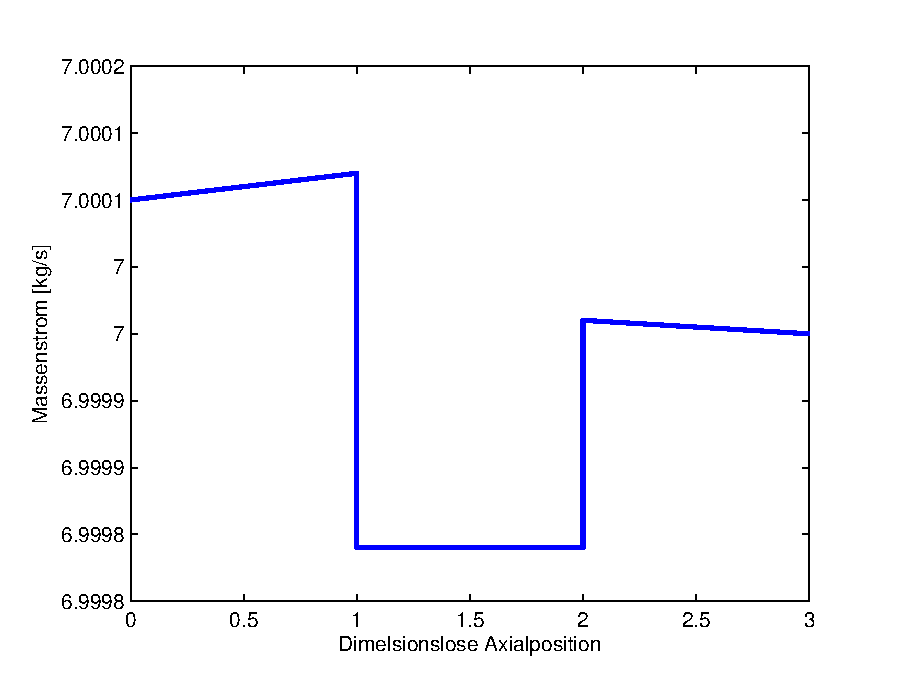
\includegraphics[width=0.8\textwidth]{massFlow_strukt_1.eps}
	\caption{Massenstrom in der Turbine, strukturiertes Gitter} \label{fig:massFlowStrukt}
\end{figure} 
 \begin{figure}[htbp]
	\centering
	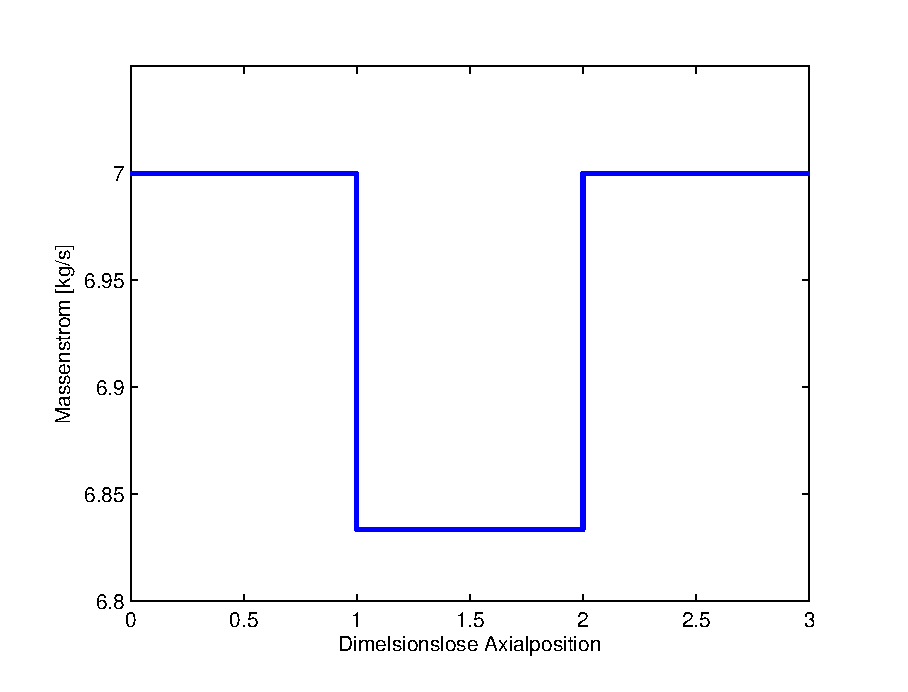
\includegraphics[width=0.8\textwidth]{massFlow_unstrukt_1.eps}
	\caption{Massenstrom in der Turbine, unstrukturiertes Gitter} \label{fig:massFlowUnstrukt}
\end{figure} 
\subsection{Wirkungsgrade mit temperaturabhängigem $c_p$}
\begin{table}[H]
	Für die Untersuchung der Wirkungsgrade unter Berücksichtigung der spezifischen Wärmekapazität in Abhängigkeit der Temperatur wurden die Definitionen aus Kapitel \ref{subsec:spezWK} verwendet. 
	Als Resultate ergeben sich die Wirkungsgrade in Tabelle \ref{tab:strukturiertmycp} und \ref{tab:unstrukturiertmycp}. Hierbei ist durchaus eine Veränderung zu beobachten, welche jedoch nur teilweise auf die nun verwendete spezifische Wärmekapazität zurückzuführen ist. Ein größerer Faktor für die Veränderung der Wirkungsgrade ist die zu beobachtenden Änderungen des Massenstroms und die unterschiedliche Definition der verwendeten Wirkungsgrade. Für die Isentrope Leistung wird immer der Massenstrom gemessen am Einlauf der Turbine verwendet, während für den Wirkungsgrad $\eta_{c_p, T_t}$ zur Berechnung der erzeugten Leistung die lokalen Massenströme an Einlauf und Auslauf verwendet werden. selbst kleine Schwankungen des Massenstroms führen hierbei zu gravierenden Änderungen im Wirkungsgrad.
	
	\centering
	\caption{Vergleich der Wirkungsgraddefinitionen auf einem strukturierten Gitter mit $c_p = f(T)$}
	\begin{tabular}{ l| c | c c c c}
		&	$c_p = const.$	&	$c_p(T)$	&		&		&		\\
		\hline
		&		&	$c_p^*$	&	$\overline{c_p^*}$	&	$\overline{c_p}$	&	$c_p$	\\
		\hline
		$\eta_{CFX}$	&	81,24 \%	&	53,89\%	&	79,19 \%	&	79,19 \%	&	60,25\%	\\
		$\eta_{c_p, T_t}$	&	81,25\%	&	74,6 \%	&	78,3 \%	&	78,07\%	&	83,41 \%	\\
	$\eta_{torque}$	&	82,52\%	&	54,35 \%	&	80,11 \%	&	79,87 \%	&	60,77\%	\\
		
	\end{tabular}
	\label{tab:strukturiertmycp}
\end{table}

\begin{table}[H]
	\centering
	\caption{Vergleich der Wirkungsgraddefinitionen auf einem unstrukturierten Gitter mit $c_p = f(T)$}
	\begin{tabular}{ l| c | c c c c}
		&	$c_p = const.$	&	$c_p(T)$	&		&		&		\\
		\hline
		&		&$c_p^*$	&	$\overline{c_p^*}$	&	$\overline{c_p}$	&	$c_p$	\\
		\hline
		$\eta_{CFX}$	&	80,21 \%	&	71,93 \%	&	77,96 \%	&	78,34 \%	&	60,01 \%	\\
		$\eta_{c_p, T_t}$	&	80,1 \%	&	\textcolor{red}{100,36} \%	&	78,23 \%	&	78,61\%	&	83,72 \%	\\
		$\eta_{torque}$	&	79,5 \%	&	70,23 \%	&	77,1 \%	&	77,48 \%	&	59,36 \%	\\
		
	\end{tabular}
	\label{tab:unstrukturiertmycp}
\end{table}
%%% Local Variables: 
%%% mode: latex
%%% TeX-master: "main"
%%% End: 


